%% paper_template.tex is a modification of:
%% bare_conf.tex
%% V1.2
%% 2002/11/18
%% by Michael Shell
%% mshell@ece.gatech.edu
%%
%% This is a skeleton file demonstrating the use of IEEEtran.cls
%% (requires IEEEtran.cls version 1.6b or later) with an IEEE conference paper.
%%
%% Support sites:
%% http://www.ieee.org
%% and/or
%% http://www.ctan.org/tex-archive/macros/latex/contrib/supported/IEEEtran/
%%
%% This code is offered as-is - no warranty - user assumes all risk.
%% Free to use, distribute and modify.

% Frank Cangialosi
% Gemstone Team Tesla
% CNAM, Department of Physics
% University of Maryland
% College Park, MD 20742
% frank@cs.umd.edu
% (410)-375-7977

\documentclass[conference]{IEEEtran}

\usepackage[usenames,dvipsnames]{xcolor}
\usepackage{cite}
\input epsf
\usepackage{graphicx}
\usepackage{caption}
\usepackage[labelformat=empty,position=top]{subcaption}
\usepackage[export]{adjustbox}

\newcommand{\sma}[1]{{\textcolor{red}{\bf sma: #1}}}
\newcommand{\frank}[1]{{\textcolor{blue}{\bf frank: #1}}}
\newcommand{\ph}[1]{{\textcolor{green}{\bf patrick: #1}}}

\newcommand{\numrange}[2]{#1--#2}

\hyphenation{op-tical net-works semi-conduc-tor IEEEtran}

\begin{document}

\title{\LARGE Time Reversed Electromagnetic Wave Propagation as a Novel Method of Wireless Power Transfer}

\author{
    \authorblockN{Frank Cangialosi, Tyler Grover, Patrick Healey, Tim Furman,
		Andrew Simon and Steven M. Anlage}
    \authorblockA{
    Gemstone Team TESLA, Center for Nanophysics and Advanced Materials, Department of Physics,\\
    University of Maryland, College Park, MD 20742-4111   USA
    }
}

\maketitle

%%%%%%%%%%%%%%%%%%%%%%%%%%%%%%%%%%%%%%%%%%%%%%%%%%%%%%%%%%%%%%%%%%%%%%%%%%%%%%%%
\begin{abstract}
We investigate the application of time reversed electromagnetic wave propagation
to transmit energy to a moving target in a reverberant environment.
%
``Time reversal'' is a signal focusing method that exploits the time reversal
invariance of the lossless wave equation to direct signals on a single point
inside a complex scattering environment.
%
In this work, we explore the properties of time-reversed microwave pulses in a
low-loss ray-chaotic chamber.
%
We measure the spatial profile of the collapsing wavefront around the target
antenna, and demonstrate that time reversal can be used to transfer energy to a
receiver in motion.
%
We discuss the results of these experiments, and explore their implications for
a wireless power transmission system based on time reversal.

\end{abstract}
%%%%%%%%%%%%%%%%%%%%%%%%%%%%%%%%%%%%%%%%%%%%%%%%%%%%%%%%%%%%%%%%%%%%%%%%%%%%%%%%

\IEEEpeerreviewmaketitle
%%%%%%%%%%%%%%%%%%%%%%%%%%%%%%%%%%%%%%%%%%%%%%%%%%%%%%%%%%%%%%%%%%%%%%%%%%%%%%%%
\section{introduction}
\label{sec:intro}

Many techniques have been proposed for wireless power transfer (WPT)
ranging from magnetic resonance to microwave beaming.
%
While the ability to transmit power practically and efficiently at short to
mid-range is well demonstrated in the literature, there is relatively little
prior work that retains both high efficiency and practicality at distances
beyond a few meters~\cite{wpt-progress}.



Traditional methods of long-range WPT have relied on microwave
beaming~\cite{history-wpt}.
%
While efficient, this technique requires precise alignment of transmitter and
receiver, and requires a clear line of sight propagation path.
%
Even in those cases where line of sight might be achievable, it is highly
impractical due to the danger it introduces to any humans or wildlife that might
cross its path.
%
Finding a way to transmit microwave power over long distances in a less 
concentrated transmission channel would be highly desirable.



Magnetic resonance beacons have been used to extend magnetic resonance coupling
to longer distances.
%
While safer than microwave beaming, these beacons still have a relatively
limited range~\cite{wpt-progress}.
%
There is also interest in MIMO (Multiple Input Multiple Output) charging devices
that allow for combined data and energy transfer using microwaves.
%
The proposed Cota system, for example, is able to wirelessly transmit power via
a form of magnetic-beamforming~\cite{mimo}.
%
Other methods, such as WattUp, apply phase conjugation to the
microwave signal~\cite{wattup}, but suffer from bandwidth
limitations in general~\cite{prada-mirror,derode-mult}.
%
The efficiency and reliability of these techniques has yet to be fully explored
in the literature.



In this paper, time reversal is proposed as a potential alternative to
the methods described above.
%
The method is especially well suited for ray chaotic environments, which are
quite commonly found in settings where WPT technology is desired~\cite{hemmady}.
%
The source sends weak signals through many different trajectories in the
scattering environment, spread out over an extended time period.
%
All of these signals converge on to the target location where they
superimpose coherently at one instant to deliver a large burst of power.
%
As a result energy is concentrated only at the location of the intended target,
and the limitations of microwave beaming are avoided.



While there exists extensive prior work on electromagnetic time
reversal~\cite{fink,nltr-wave-chaotic,nltr-classical-waves,tr-green}, it remains
largely unexplored in the context of WPT\@.
%
For the technique to be viable, reconstructions must converge in a small region,
without interfering with nearby electronics or biological matter.
%
Here we employ a very elementary single-channel time reversal mirror to
accomplish this task.



The primary advantage of time reversal in the context of wireless power transfer
is its ability to locate a target object anywhere in an enclosed space, well
beyond the meter scale between source and
receiver~\cite{fink,nltr-wave-chaotic}.
%
This overcomes the main distance limitation imposed by technologies relying
on magnetic near fields.



This paper explores the ability of time reversal to focus energy on a point in
space.
%
The size of the reconstruction region on the target is quantified, and a fit to
the spatial distribution of energy is introduced as a function of carrier signal
wavelength.
%
Time reversed energy collapse is demonstrated on a moving target, and a model is
similarly generated describing the energy delivered to the moving system.
%
These models are defined in terms of the parameters of the system and the
theoretical bounds are discussed.
%%%%%%%%%%%%%%%%%%%%%%%%%%%%%%%%%%%%%%%%%%%%%%%%%%%%%%%%%%%%%%%%%%%%%%%%%%%%%%%%

%%%%%%%%%%%%%%%%%%%%%%%%%%%%%%%%%%%%%%%%%%%%%%%%%%%%%%%%%%%%%%%%%%%%%%%%%%%%%%%%
\section{Methodology}
\label{sec:methodology}


\begin{figure}[]
	\centering
	\begin{subfigure}[t]{0.03\columnwidth}
	\textbf{(a)}
	\end{subfigure}
	\begin{subfigure}[t]{0.9\columnwidth}
		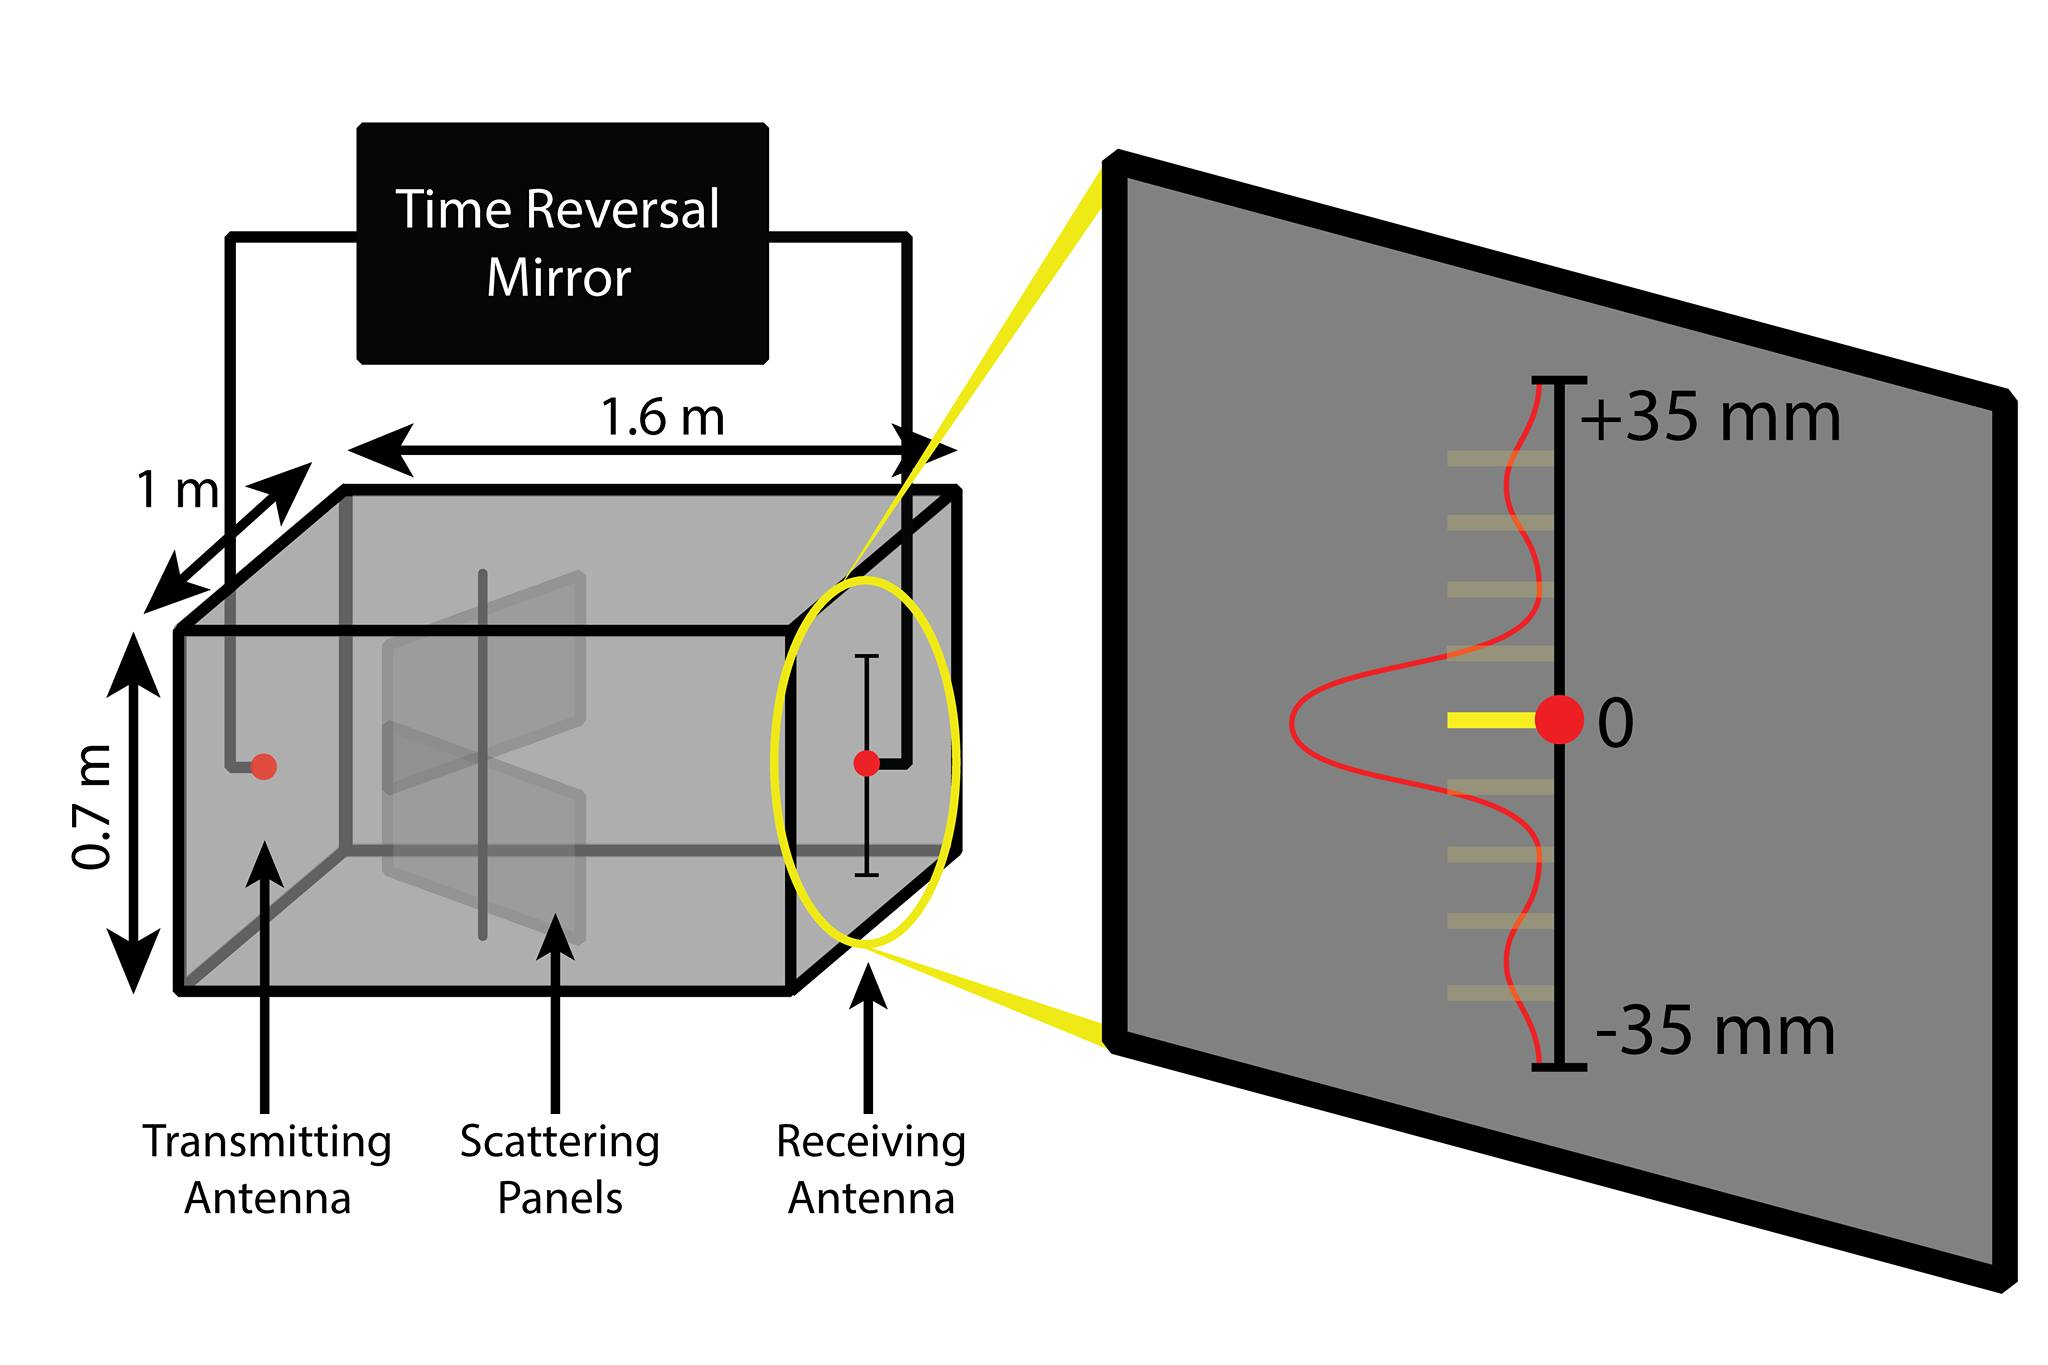
\includegraphics[width=\columnwidth,valign=t]{figs/gigabox.jpg}
		\caption{\label{fig:gigabox}}
	\end{subfigure}
	\begin{subfigure}[]{0.9\columnwidth}
		\vspace{-1.5\baselineskip}
	\begin{subfigure}[t]{0.03\columnwidth}
	\textbf{(b)}
	\end{subfigure}
		\begin{subfigure}[t]{0.45\columnwidth}
				\centering
				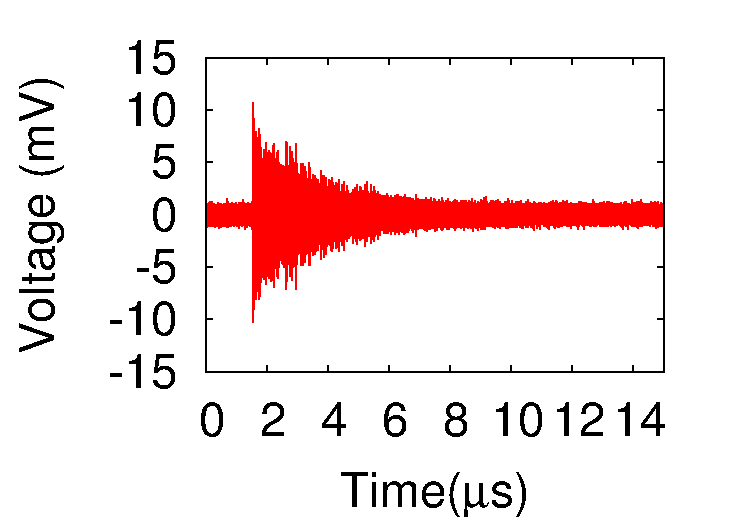
\includegraphics[width=\columnwidth,valign=t]{figs/sona.pdf}
				\caption{\label{fig:sona}}
		\end{subfigure}
	\begin{subfigure}[t]{0.03\columnwidth}
	\textbf{(c)}
	\end{subfigure}
		\begin{subfigure}[t]{0.45\columnwidth}
				\centering
				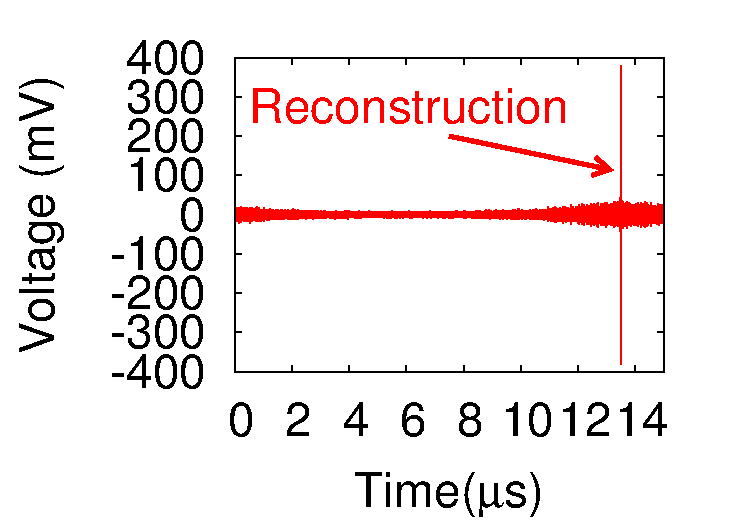
\includegraphics[width=\columnwidth,valign=t]{figs/recon.pdf}
				\caption{\label{fig:recon}}
		\end{subfigure}
	\end{subfigure}
  \vspace{-1\baselineskip}
	\caption{(a): A ray-chaotic enclosure with two antennas, one of
	which is attached to a sliding panel that can move freely along the $y$-axis,
	as shown in the right inset. A time-reversed sona (b) is broadcast from the
	transmitting antenna, resulting in a reconstruction at the receiving
	antenna, shown in (c).}
	\label{fig:setup}
\vspace{-0.5\baselineskip}
\end{figure}


\subsection{Experimental Setup}

We have investigated the applicability of time reversal to wireless power
transfer within an enclosed, reflective cavity (Fig.~\ref{fig:gigabox}): a
1.06~$m^3$ aluminum box with a conductive scattering paddle to make the ray
trajectories more ergodic.
%
Ray chaos ensures that a propagating pulse will eventually reach every point in
the environment, which insures that many transmission channels are
simultaneously excited, and this improves reconstruction fidelity.
%
The basic time reversal process in this environment proceeds as follows: First,
a 50~ns Gaussian pulse (with a carrier frequency of 5~GHz) is injected into
the cavity through the transmitting antenna.
%
A complex signal (referred to as a ``sona'') is measured at the receiving
antenna (Fig.~\ref{fig:sona}).
%
This sona is the sum of the reflections of the initial pulse, scaled in
magnitude due to ray-divergence and loss, and shifted in time due to differing
lengths of reflection paths.
%
In the next step, this sona is time reversed and injected into the transmitting
antenna.
%
The result is a reconstruction of the initial pulse back at the receiving
antenna (Fig.~\ref{fig:recon}).
%
This process makes use of another robust symmetry, namely the spatial
reciprocity of the wave equation.



Two monopole antennas inject and extract electromagnetic signals from different
points in the enclosure. A transmitting antenna is attached to the cavity wall
opposite the receiving antenna.
%
The receiving antenna is attached to a panel that can move vertically with a
total range of 70~mm.
%
Motion of the receiving antenna is achieved using an externally-mounted PI
MikroMove \texttt{M-415.DG} translation stage and the enclosure remains sealed
during the translation.



Interrogation pulses and time-reversed sona signals are created and broadcast
using a \texttt{Tektronix AWG7052} arbitrary waveform generator feeding an
\texttt{Agilent E8267D} Vector PSG microwave source.
%
A digital storage oscilloscope (DSO, \texttt{Agilent DSO91304A}) is used to
record waveforms of interest. MATLAB is used for signal processing and
instrument control and coordination.
%%%%%%%%%%%%%%%%%%%%%%%%%%%%%%%%%%%%%%%%%%%%%%%%%%%%%%%%%%%%%%%%%%%%%%%%%%%%%%%%

%%%%%%%%%%%%%%%%%%%%%%%%%%%%%%%%%%%%%%%%%%%%%%%%%%%%%%%%%%%%%%%%%%%%%%%%%%%%%%%%
\section{Results}


\begin{figure}[t!]
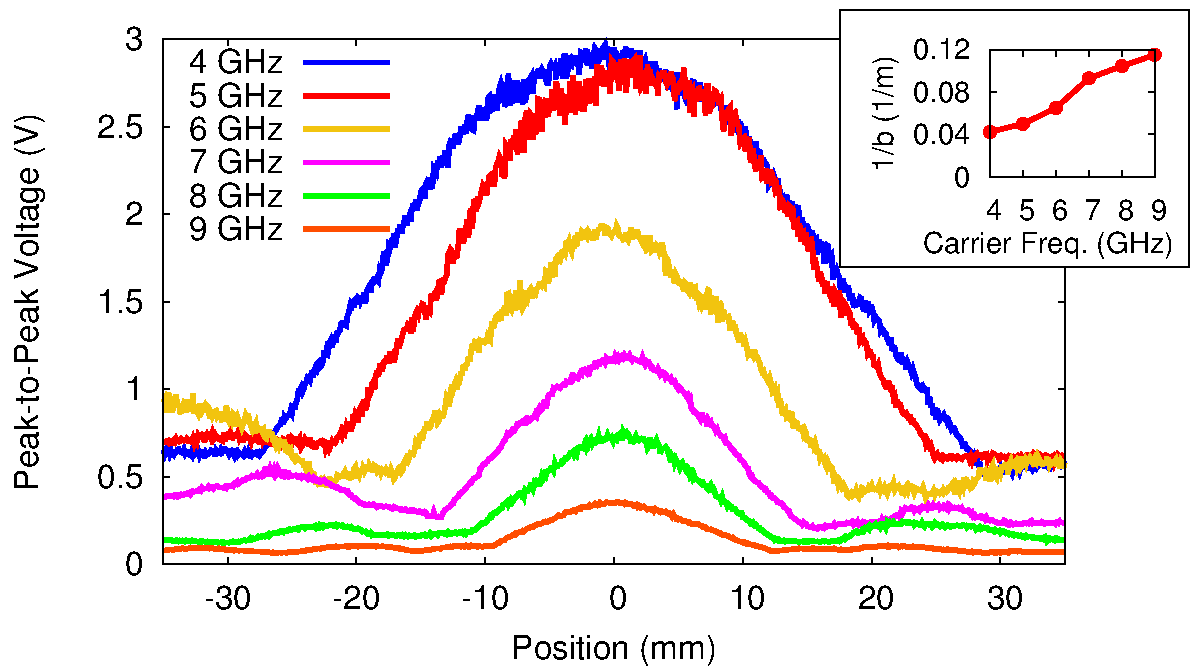
\includegraphics[width=\columnwidth]{figs/freq_profile.pdf}
\caption{Spatial profile of peak-to-peak voltage amplitudes of reconstructions 
at carrier frequencies ranging from \numrange{4}{9}~GHz in 1~GHz
steps. The inset shows the inverse of the fit $b$ value versus carrier
frequency, showing the expected linear relationship. Differences in amplitude
are due to differences in $S_{1,2}$ parameters between frequencies for our particular antennas.}
\label{fig:freq_profile}
\end{figure}


%%%%%%%%%%%%%%%%%%%%%%%%%%%%%%%%%%%%%%%%%%%%%%%%%%%%%%%%%%%%%%%%%%%%%%%%%%%%%%%%
\subsection{Spatial Profiling}
\label{sec:spatial}

The first experiment conducted measures the spatial profile of a reconstruction,
with the goal of characterizing reconstruction size as a function of carrier
signal wavelength.
%
A reconstruction is focused on the receiving antenna, in the middle of its
movement range.
%
Without changing the time reversed sona being broadcast, the receiving antenna
is systematically translated through its entire range of movement.
%
Samples are taken every 0.2~mm across the entire 70~mm range, and the
maximum peak-to-peak voltage of the corresponding reconstruction is recorded at
each step.
%
We repeated this experiment for carrier frequencies in the range
\numrange{4}{9}~GHz and display these results in Fig.~\ref{fig:freq_profile}.



The reconstruction peak-to-peak voltage profile is expected to take the form of
a \texttt{|sinc(x)|} function about the antenna~\cite{lerosey-focusing}.
%
Thus, the following equation is proposed to predict $V(x)$, the maximum
peak-to-peak voltage from a given reconstruction, as a function of $x$, the
distance between the reconstruction focal point and the receiver:
%
\begin{equation}\label{eq:vx}
V(x)=a\cdot \left|sinc\left(\frac{x+c}{b}\right)\right|+d\,,
\end{equation}
%
\noindent where $a$ is the maximum peak-to-peak reconstruction amplitude, $b$ is
the wavelength of the signal divided by $2\pi$, $c$ is the location of the
antenna along the $x$-axis, and $d$ is the noise-level offset voltage.



Since $b$ is proportional to the wavelength (and inversely proportional to
frequency), as the carrier frequency is increased, $\frac{1}{b}$ also increases,
causing the main lobe of the \texttt{|sinc(x)|} function in
Fig.~\ref{fig:freq_profile} to get smaller.
%
This relationship is shown explicitly in the inset of
Fig.~\ref{fig:freq_profile}.



Fig.~\ref{fig:error_fit} shows Equation~\ref{eq:vx} fit to the 5~GHz curve from
Fig.~\ref{fig:freq_profile}, including error bars.
%
The fit is good, but has a reduced $\chi^2$ of $234$ due in part to the rather
large background noise level.
%
The error bars are primarily systematic, introduced by the oscilloscope internal
voltage multiplier used in scaling.
%%%%%%%%%%%%%%%%%%%%%%%%%%%%%%%%%%%%%%%%%%%%%%%%%%%%%%%%%%%%%%%%%%%%%%%%%%%%%%%%

%%%%%%%%%%%%%%%%%%%%%%%%%%%%%%%%%%%%%%%%%%%%%%%%%%%%%%%%%%%%%%%%%%%%%%%%%%%%%%%%
\subsection{Moving Reconstructions}
\label{sec:moving}


\begin{figure}[t!]
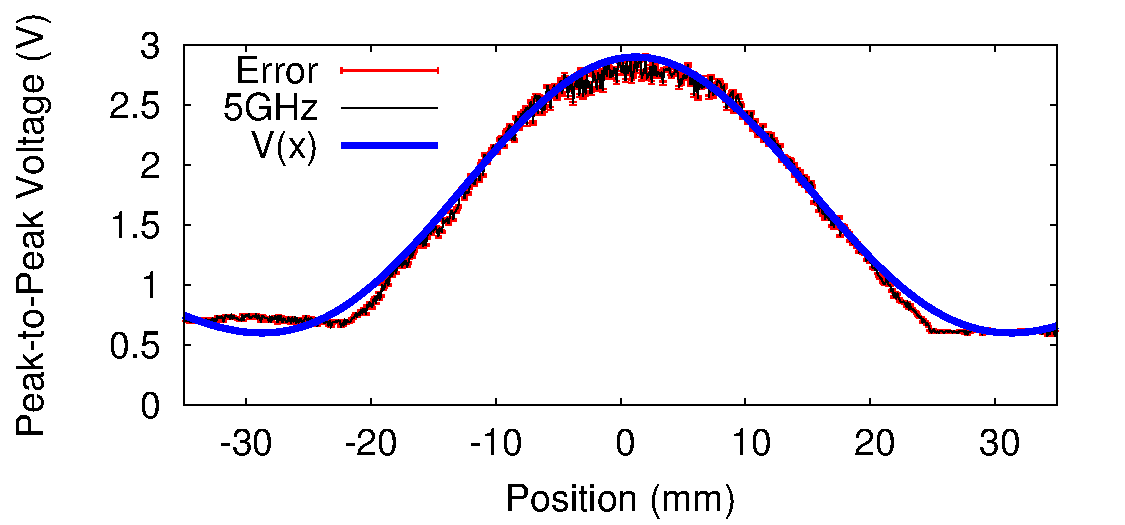
\includegraphics[width=\columnwidth]{figs/fit.pdf}
\caption{Measured peak-to-peak voltage amplitude of reconstructions received in the
vicinity of a time-reversed wave collapse location with a 5 GHz carrier
frequency, and fit to Eq.~\ref{eq:vx}}
\label{fig:error_fit}
\end{figure}


The time reversal process assumes that the environment remains fixed between the
time-forward and time-reversed steps.
%
It also assumes that the source and target remain fixed between these two steps.
%
We performed time reversal on a moving target to better understand how a
translating target affects reconstruction strength.



For this experiment, the receiving antenna moved at a constant speed of
0.5~$\frac{mm}{s}$ across the entire 70~mm range provided by the MikroMove.
%
To counteract the degradation of reconstruction strength as the antenna moved,
we periodically repeated the interrogation step, effectively re-centering the
reconstruction on the antenna.
%
Since the test equipment does not allow broadcast of one sona while collecting
another, it was not possible to transmit power during the collection time,
leading to a finite ``dead time'', denoted $t_d$ in Fig.~\ref{fig:moving_recon}.
%
During the broadcast period, the time-reversed sona was continually broadcast
into the cavity (once every 15~$\mu s$) and the peak-to-peak voltage across the
receiver was measured once every 2.05~seconds, meaning that the reconstructions
are highly under-sampled in this plot.
%
After every 15~samples were collected, we paused to collect a new sona and
repeated the process. We refer to this full process of collecting a new sona and
then broadcasting it for a given period time as a full ``cycle'' of length
$t_c$.
%
The results in Fig.~\ref{fig:moving_recon} were obtained using a carrier
frequency of 5~GHz, $t_d$ of 7~seconds, and $t_c$ of 39.8~seconds.



Based on the results from Section~\ref{sec:spatial}, the peak-to-peak
reconstruction voltage measured by the receiver is expected to decay according
to the \texttt{|sinc(x)|} function as the receiver moves away from the
reconstruction focal point.
%
This \texttt{|sinc(x)|} function will be centered on the position where the sona
was last collected, making the reconstruction focus continually lag behind the
antenna.
%
Consequently, the maximum reconstruction strength is limited by the time needed
to collect, time reverse and re-broadcast an updated sona.



The following equation is proposed as a model for the peak-to-peak voltage of
the reconstruction on a moving target as a function of time, assuming a constant
velocity $\bar{v}$:
%
\begin{equation}\label{eq:vt}
  V(t) = \left\{
        \begin{array}{lr}
                0 & : t\pmod{t_c} \le t_d \\
                a\cdot \left|sinc\left(\frac{\bar{v}t}{b}\right)\right|+d & : t\pmod{t_c} > t_d
        \end{array}\,.
  \right.
\end{equation}



In Fig.~\ref{fig:moving_recon}, the green curve represents a fit of
Equation~\ref{eq:vt} to one full cycle. As in Fig.~\ref{fig:error_fit}, this
function fits the data well using the same parameters.



\begin{figure}[t]
\centering
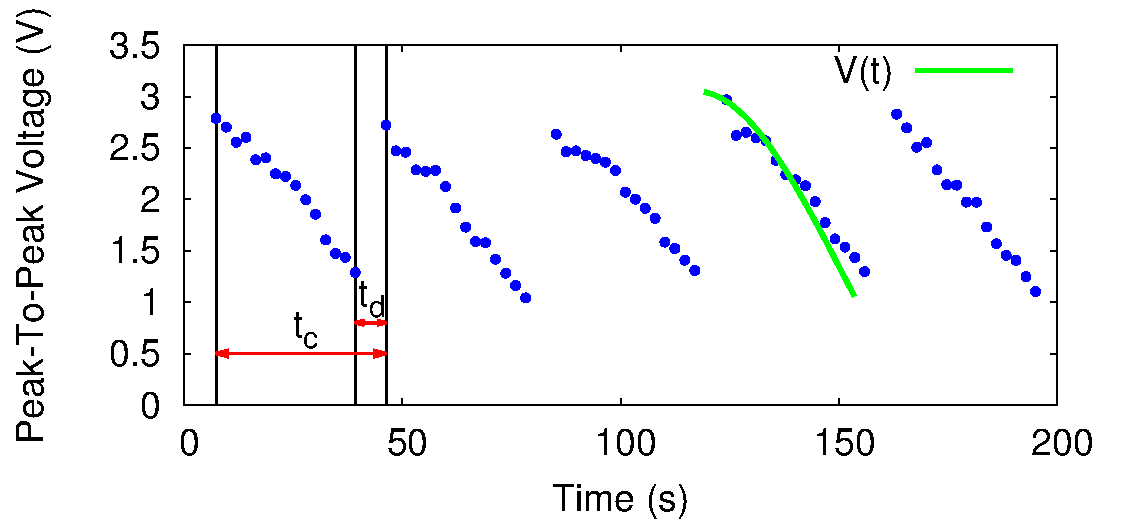
\includegraphics[width=\columnwidth]{figs/moving_recon.pdf}
\caption{Reconstruction voltage amplitude vs.\ time as the target moves along
one wall of the enclosure. A new sona signal is acquired every $t_{c}=39.8s$,
leading to a dead time of duration $t_{d}=7s$. The target is moving at a speed
of 0.5~$\frac{mm}{s}$ and the carrier frequency is 5~GHz.}
\label{fig:moving_recon}
\end{figure}
%%%%%%%%%%%%%%%%%%%%%%%%%%%%%%%%%%%%%%%%%%%%%%%%%%%%%%%%%%%%%%%%%%%%%%%%%%%%%%%%

%%%%%%%%%%%%%%%%%%%%%%%%%%%%%%%%%%%%%%%%%%%%%%%%%%%%%%%%%%%%%%%%%%%%%%%%%%%%%%%%
\section{Discussion}
\label{sec:discussion}

%%%%%%%%%%%%%%%%%%%%%%%%%%%%%%%%%%%%%%%%%%%%%%%%%%%%%%%%%%%%%%%%%%%%%%%%%%%%%%%%
\subsection{Proposed TR WPT System}
\label{sec:system}

This research represents a first step in the exploration of a WPT system based on TR. We now propose a potential proof-of-concept system based on our findings in Fig.~\ref{fig:SysImage}. In this work, we investigate one particular performance parameter of the system. However, many unknowns regarding the design and performance of a complete system remain.

The proposed system has two basic components. The first is a rectenna that serves as the receiver. Although the system as described in Section~\ref{sec:meth} would require an out-of-band feedback channel between the receiver and transmitter, prior work has shown how a transmitter can target  receivers entirely in-band~\cite{nltr-wave-chaotic,roman}. Our system in Fig.~\ref{fig:SysImage} builds on these findings.

The second component is a transmitter that performs the time reversal process. This system will record identifying signals from the receiver(s), time reverse the signals, and re-broadcast them into the environment.

Although not a component of the system, another important consideration in building a WPT system based on TR is the environment, as TR is heavily dependent on environmental factors. A low-loss scattering environment is necessary for the technique to be effective.

\subsection{Contributions and Future Work}
\label{sec:contrib}

In the above experiments, we demonstrate the shape of the spatial profile of an electromagnetic
time-reversed collapse. This profile takes the form \texttt{|sinc(x)|}, dependent on wavelength $b$.
Additionally, the ability of a TR system to transmit energy to a moving target is
demonstrated to be dependent on the spatial profile and transmission dead
time $t_{d}$.

Any WPT system utilizing time reversal will have to account for the
finite-size bubble of fields around the main reconstruction point.
Methods have been developed to improve the spatial focusing of reconstructions
well below the diffraction limit~\cite{lerosey-focusing}.

Based on the results shown in Fig.~\ref{fig:moving_recon}, it is clear that a faster
processing speed is required to track a moving target.
%
Nevertheless, we believe one of the main advantages of time reversal over
existing WPT methods is its ability to track moving
targets~\cite{fink,nltr-wave-chaotic}.


\begin{figure}[t]
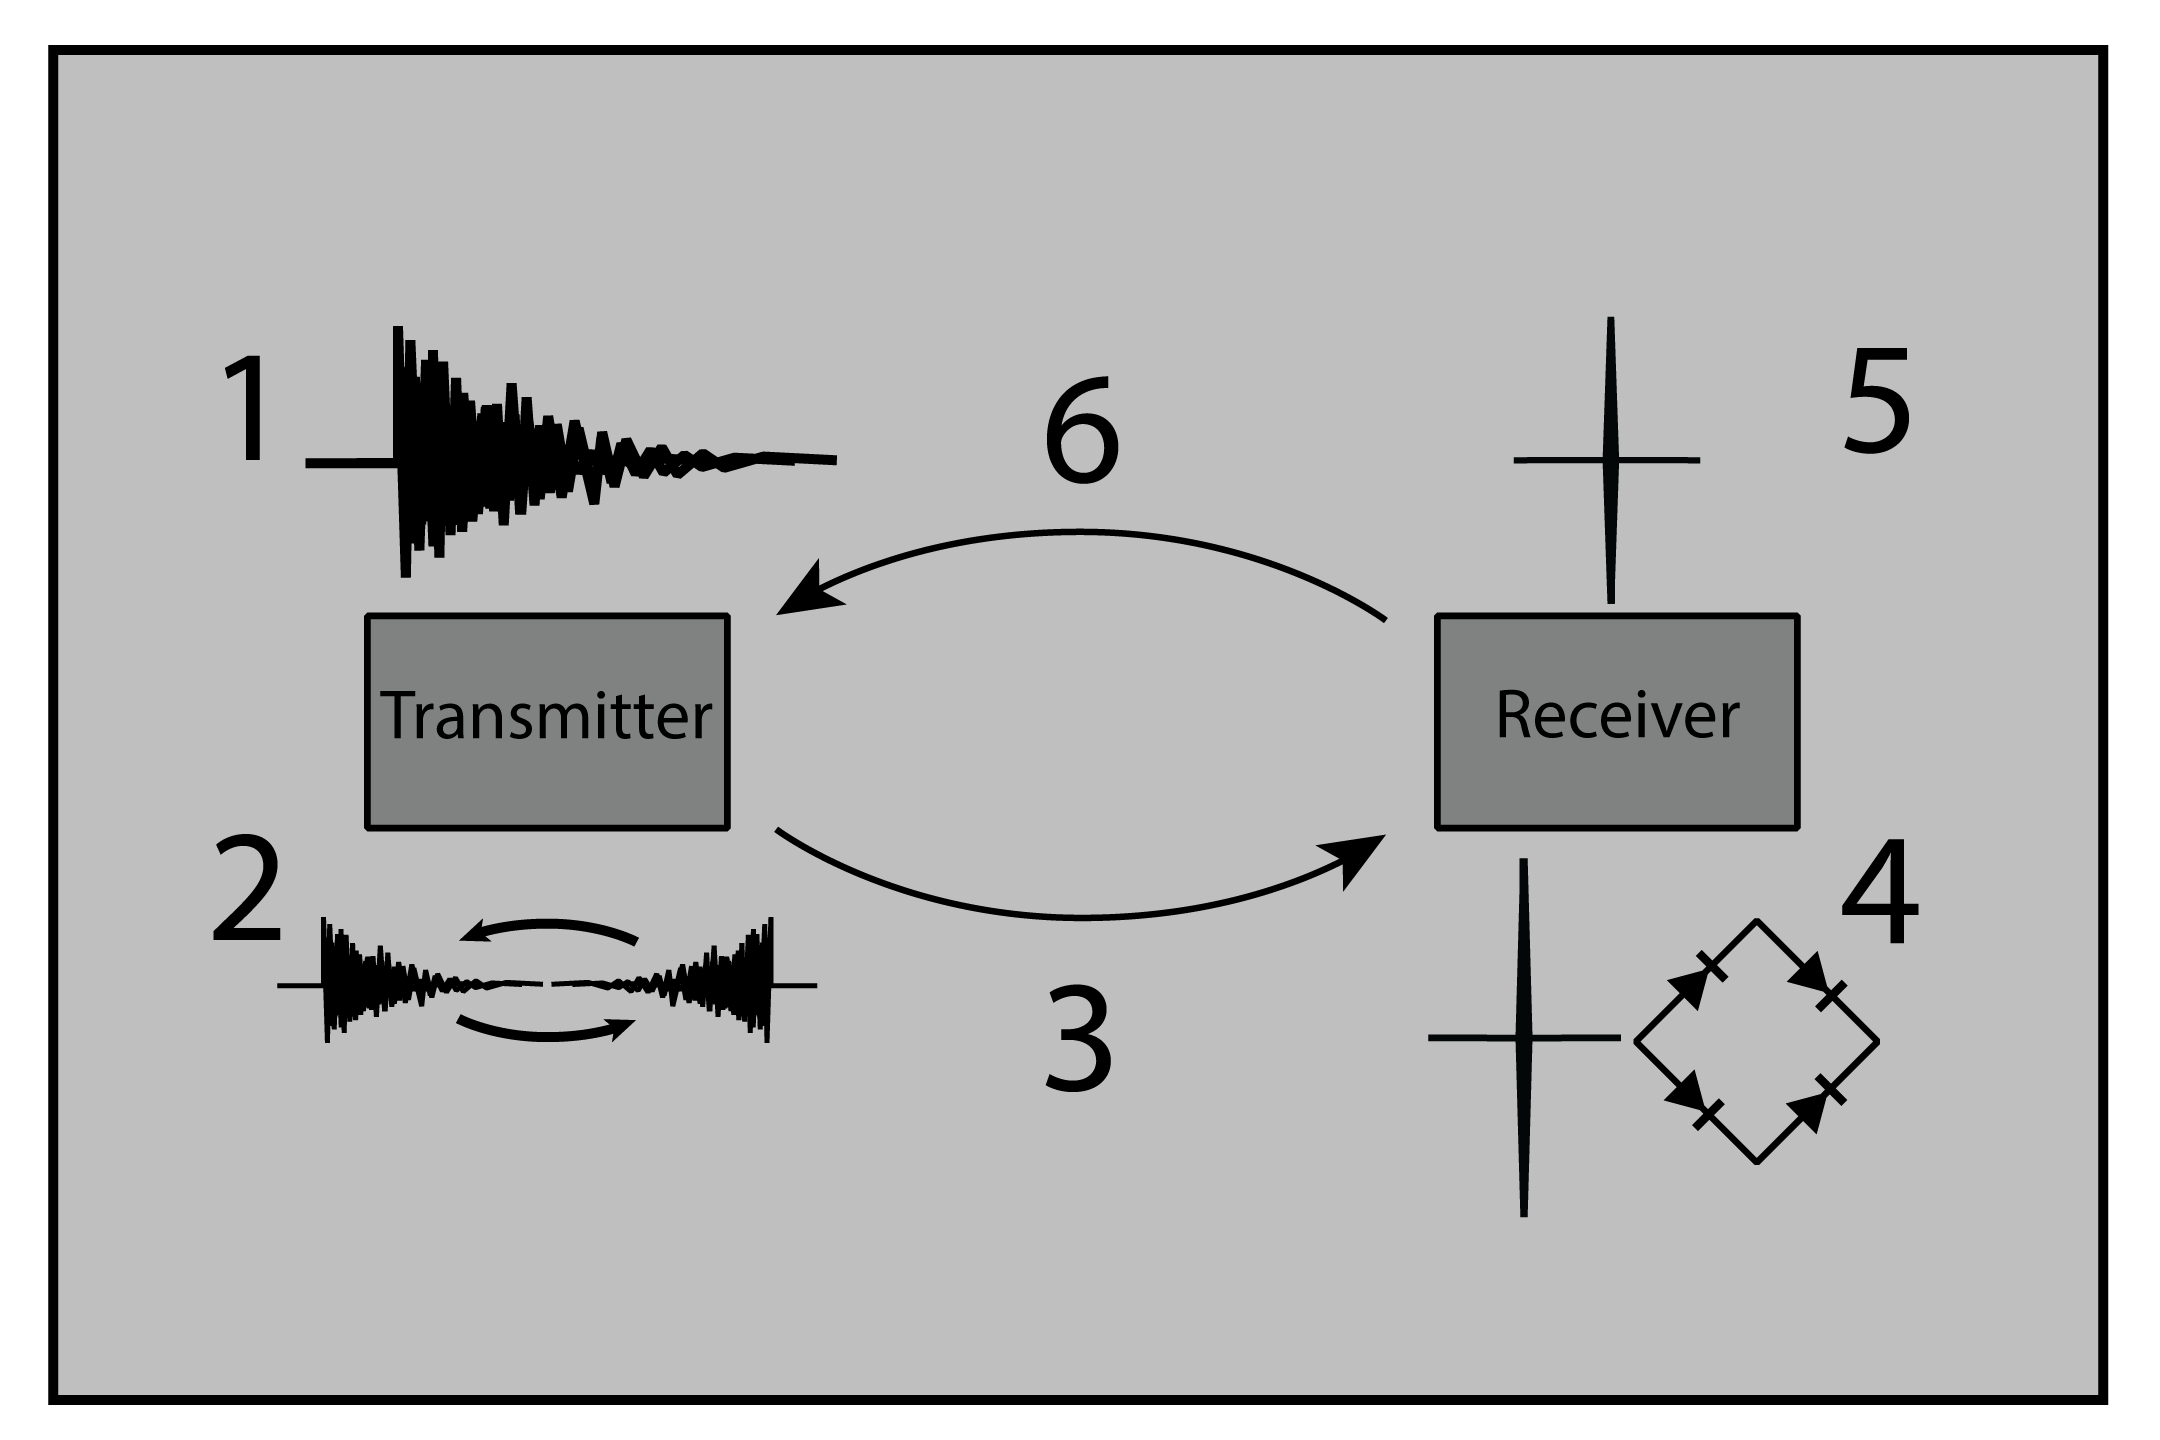
\includegraphics[width=\columnwidth]{figs/WPTSys.png}
\caption{A notional time reversal wireless power transfer system. A new receiver joins the system by broadcasting or emitting a characteristic signal (0). The next sona that the transmitter collects will contain spatial information leading back to this receiver (1). In the power transfer cycle, the sona is time-reversed (2) and broadcast back into the environment. An amplified version of the signal reconstructs on the receiver (3), which rectifies the energy (4). A small amount of the energy is used to broadcast a new signal (5) into the environment, which will be collected in the next sona (6). The cycle repeats from (2).}
\label{fig:SysImage}
\end{figure}
%%%%%%%%%%%%%%%%%%%%%%%%%%%%%%%%%%%%%%%%%%%%%%%%%%%%%%%%%%%%%%%%%%%%%%%%%%%%%%%%

%%%%%%%%%%%%%%%%%%%%%%%%%%%%%%%%%%%%%%%%%%%%%%%%%%%%%%%%%%%%%%%%%%%%%%%%%%%%%%%%
\subsection{Limitations}
\label{sec:limitations}


These experiments were limited primarily by the environment and equipment used
for testing.
%
A consumer electronics environment is likely to be much larger than the chamber
used in this study, and filled with clutter.
%
Both of these properties would improve the modal density of the environment,
creating more transmission channels between source and target, ultimately
improving reconstruction quality.
%
On the other hand, such environments would likely have significantly larger loss
than those considered in our experiments. We found that approximately \ph{X}\% of energy transmitted through our test cavity was lost due to absorption. Understanding and characterizing how environmental factors impact TR is a major obstacle to the design of a TR WPT system. Environmental effects should be a major research priority accordingly.

%Our results show that time reversal mirrors may be able to effectively
%exploit multiple channels, but we leave this to future work.
%Great benefit can also be achieved by utilizing multi-channel time reversal mirrors.
%Understanding how
%to maximize the effectiveness of these technologies while minimizing cost is
%critical.

The single-channel time reversal method is limited in the amount of power it can
transmit to a target.
%
It is certainly sufficient to perform long-term trickle charging or to act as a
secondary-source of energy extending battery life.
%
A multi-channel realization of time reversal will be able to deliver much
greater time-integrated power.



The theoretical limit for the speed of the time reversal process needs to be
determined.
%
These experiments were severely limited by the processing time of the combined
MATLAB-DSO-AWG-PSG test and measurement system.
%
Dedicated hardware and firmware would eliminate communication overhead and thus
dramatically improve the speed of the WPT process presented here.
%%%%%%%%%%%%%%%%%%%%%%%%%%%%%%%%%%%%%%%%%%%%%%%%%%%%%%%%%%%%%%%%%%%%%%%%%%%%%%%%

%%%%%%%%%%%%%%%%%%%%%%%%%%%%%%%%%%%%%%%%%%%%%%%%%%%%%%%%%%%%%%%%%%%%%%%%%%%%%%%%
\section{Conclusion}


This paper proposes time reversed electromagnetic wave propagation as a new
approach for WPT.
%
Our experiments demonstrate that the spatial profile of reconstruction voltage
is very tightly confined to the area surrounding the intended receiving antenna,
and follows a $\left|sinc(x)\right|$ profile.
%
Further, we successfully demonstrate the ability to focus time reversed signals
onto a moving target in a ray-chaotic scattering environment.
%
We believe that, with improvements to the transmitter and receiver, time reversal
could provide a viable approach for WPT in certain environments.
%%%%%%%%%%%%%%%%%%%%%%%%%%%%%%%%%%%%%%%%%%%%%%%%%%%%%%%%%%%%%%%%%%%%%%%%%%%%%%%%

%%%%%%%%%%%%%%%%%%%%%%%%%%%%%%%%%%%%%%%%%%%%%%%%%%%%%%%%%%%%%%%%%%%%%%%%%%%%%%%%
\section*{Acknowledgments}
This work was supported by ONR through grant \#N000141512134, the UMD Gemstone
program, and CNAM. 
%
We would like to acknowledge all members of Gemstone Team TESLA for their
feedback on results and data used in this paper.
%%%%%%%%%%%%%%%%%%%%%%%%%%%%%%%%%%%%%%%%%%%%%%%%%%%%%%%%%%%%%%%%%%%%%%%%%%%%%%%%


%%%%%%%%%%%%%%%%%%%%%%%%%%%%%%%%%%%%%%%%%%%%%%%%%%%%%%%%%%%%%%%%%%%%%%%%%%%%%%%%
\bibliographystyle{IEEEtran}
\bibliography{bibliography}
%%%%%%%%%%%%%%%%%%%%%%%%%%%%%%%%%%%%%%%%%%%%%%%%%%%%%%%%%%%%%%%%%%%%%%%%%%%%%%%%

\end{document}
